\documentclass[a4paper, pdftex, ngerman, 11pt]{article}
\usepackage[utf8]{inputenc}
\usepackage[T1]{fontenc}
\usepackage{babel}

%\usepackage{hyperref} % Für klickbare Referenzen
\usepackage{graphicx}
\usepackage{float}

\begin{document}
\section{Warum heißt der Pinguin \emph{"`Pinguin"'}?}
\subsection{Erklärung 1}
Ursprünglich kommt der Name aus dem walisischen und heißt dort \emph{'Pen Gwyn'} (gesprochen wie das englische penguin). Es bedeutet soviel wie \emph{'Weißer Kopf'}. Seeleute aus \textbf{Wales} sollen die Tiere als erste gesehen und so genannt haben (siehe dazu Bild \ref{img:pen}).

\begin{figure}[H]
	\begin{center}
		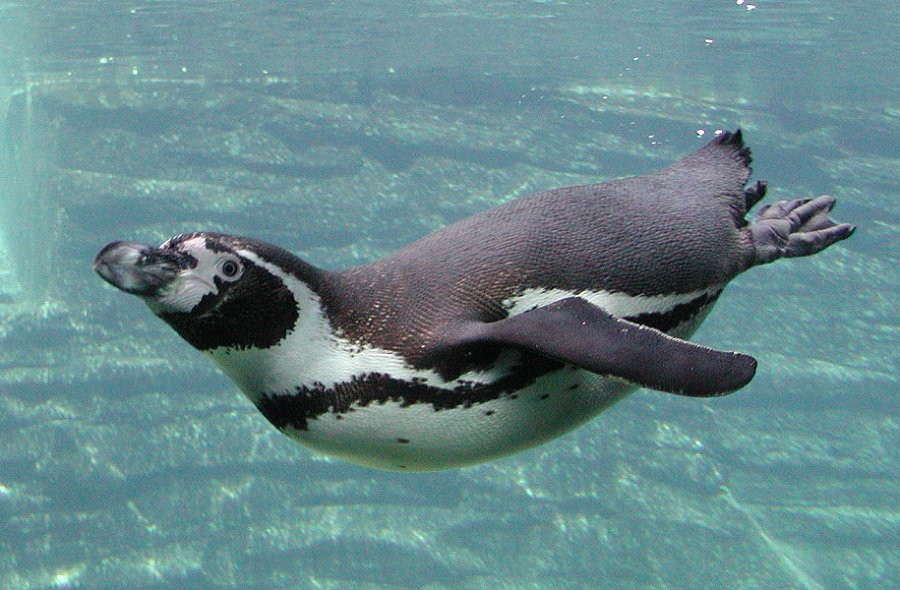
\includegraphics[width=4cm]{bilder/swim-Ping.jpg}
		\caption{Ein lebendes Exemplar eines Pinguins}
		\label{img:pen}
	\end{center}
\end{figure}

\subsection{Erklärung 2}
Es heißt aber auch, dass ursprünglich der Name \emph{'Pinguin'} eine Bezeichnung für den 1844 ausgestorbenen, ebenfalls flugunfähigen \textbf{Riesenalk} der Nordhalbkugel war (siehe Bild \ref{img:auk}).

\begin{figure}[H]
\begin{center}
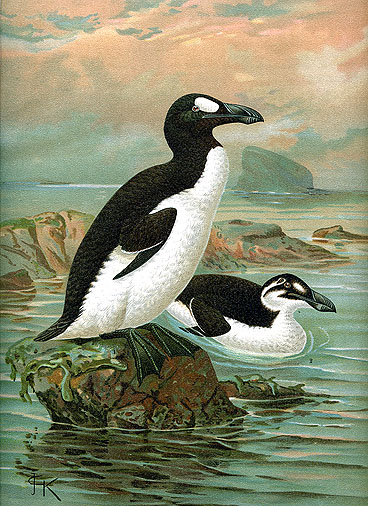
\includegraphics[width=5cm]{bilder/GreatAuk.jpg}
\caption{Ein lebendes Exemplar eines Pinguins}
\label{img:auk}
\end{center}
\end{figure}

\subsection{Erklärung 3}
Eine andere These lautet, dass der Name vom lateinischen \emph{"`penguis"'} stammt. Dies bedeutet \emph{"`Fett"'} und für die Seefahrer war Fett sehr wichtig und es ließ sich aus den \textbf{Pinguinen} gewinnen (siehe Bild \ref{img:tux}).

\begin{figure}[H]
\begin{center}

\includegraphics[width=5cm]{bilder/tux.png}
\caption{Der kleine Tux}
\label{img:tux}
\end{center}
\end{figure}

\end{document}
